%!TEX program = xelatex
\documentclass[tikz, border=3mm]{standalone}
\usepackage{pgfplots}
\usepackage{xcolor}
\usepgfplotslibrary{colormaps}
\pgfplotsset{
    compat=1.18,
    trig format plots=rad,  % 启用弧度制
    colormap/spring
}

\begin{document}
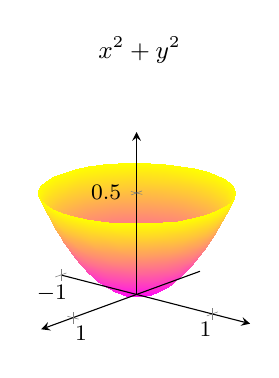
\begin{tikzpicture}
    \begin{axis}[
        title={$x^2+y^2$},     % 中文标题支持
        view={130}{25},
        axis lines=center,
        xmax=1.5, ymax=1.5, zmax=0.8,
        width=6cm, height=5cm,
        tick label style={font=\footnotesize},
        axis on top,
        title style={font=\small}    % 标题字号调整
    ]
        \addplot3 [
            surf,
            z buffer=sort,
            samples=25,             % θ方向采样
            samples y=40,           % φ方向采样
            domain=0:1,             % 半径范围
            y domain=0:2*pi,        % 角度范围
            shader=interp
        ] (
            {x*cos(y)},             % 极坐标转换
            {x*sin(y)},
            {0.5*x^2}               % 抛物面方程
        );
    \end{axis}
\end{tikzpicture}
\end{document}